\section{System Overview}
\label{sec:overview}
PriOIDC allows user to conduct single sign on with out leaking login information to IdP. And even multi RPs' collusion can not trace the user. In this section, we are going to make an overview of our user privacy respecting protocol based on OpenID Connect 1.0.
 
\subsection{Anonymity in OpenID Connect System}
%单点登录系统中,IdP通过用户认证识别用户身份,通过client_id和redirect_uri识别RP身份。
%在不改变单点登录系统结构的情况下,由于IdP要向RP提供用户的身份信息,所以向IdP隐藏用户身份是不可行的
%向IdP隐藏RP身份要通过隐藏client_id和redirect_uri实现
%The ability of IdP. Discribe the solution of protecting users' privacy.
In OpenID Connect systems IdP gets RP's identity by client\_id or redirect\_uri in request (Figure~\ref{fig:OpenID} step 2) and gets user's identity when authenticating the user (Figure~\ref{fig:OpenID} step 3). 
As IdP has to provide RP a user's authenticator bound with user's identity, it's not possible to keep user anonymous in IdP without modifying the structure of current SSO system. 
So it is only feasible to protect user's privacy by keeping RP anonymous in IdP. But it introduces new challenges.

\subsubsection{Challenges}
%最直接的隐藏RP的方法是在登录过程中使用随机的client_id与redirect_uri
%简单的修改会带来两个方面的问题:流程问题与安全问题 
%流程问题:IdP只识别注册过的client_id与redirect_uri;client_id与uid绑定,随机的client_id使每次的uid都不同
%安全问题:随机的client_id导致了不同RP之间的token可以混用;随机的redirect_uri导致IdP无法保证token只发送给对应的RP
%Security problems. The secure rules of sso system summarized from the previous research. And the simple solution will disobey which rules.
%Function problems. How the simple solution make the sso system failed.
%描述为何不能用户匿名
The simplest way to make RP anonymous in IdP is using random client\_id and redirect\_uri in each authentication. But the simple method will introduce some problems in two fields. 

%关键句子表明问题的分类
Using random client\_id and redirect\_uri results in the failure of authentication. In OpneID Connect system, IdP only accepts a request when the client\_id and redirect\_uri have been registered at IdP. So IdP will drop the request with random client\_id and redirect\_uri, in another word unregistered parameters, as the invalid request. Additionally to protect user's privacy from RPs' collusion attack, it's required that IdP should provide different user\_ids for different RPs\cite{OpenIDConnect}. It means that user\_id is bound to client\_id, so random client\_id means the user\_id is random too. As RP wants to provide a user personalize service it must identify a user with a constant identity. So randomness of client\_id is not appropriate for widely used SSO systems.  

In the other field, anonymous RP with random client\_id and redirect\_uri causes secure problems. To avoid the misuse of id\_token among different RPs, RP checks the validation of id\_token. An client\_id represents a specific RP's identity, a id\_token with this client\_id is only valid in this specific RP. But when using a random client\_id, different RPs may share the same client\_id. When a user log in a malicious RP, this RP possibly logs in other RPs with the user's id\_token if they have the same client\_id. Additionally redirect\_uri is the address where RP waits for the id\_token. Before issuing a id\_token, IdP will check the validation of redirect\_uri to avoid attacker getting the id\_token. If the redirect\_uri is random, IdP can no more protect user from sending id\_token to an attacker.
\subsubsection{Solutions against the problems}
%通过协商生成client_id,任何一方无法控制client_id的生成
%用户代理控制token的发送,保证发送给对应的RP
%使用OpenID Connect 1.0的动态注册功能保证client_id与redirect_uri的有效性
%设计client_id与user id 的生成算法,使RP能够识别用户
With dynamic registration, a RP can register new random client\_id and redirect\_uri before sending a request to IdP for id\_token. And to avoid IdP finding out RP's identity through dynamic registration, the requirement of registration token is omitted. IdP will delete the expired registration to reduce storage stress.

To identify a user in different logins, RP must have the ability to transform the user\_id provided by IdP into a constant user identity for each user. Most of current SSO system generate user\_id as a random  character string. So a new user-id-generating algorithm has to be created for user authentication. As user\_id is required to be bound to random client\_id to protect from RPs' collusion, client\_id should be the primary input parameter to user-id-generating algorithm. To make user\_id able to be transformed into a constant user identity, it is a feasible way that generating client\_id through a client-id-generating algorithm. The user-id-generating algorithm and client-id-generating algorithm will be described detailedly in Section~\ref{sec:protocol}. 

Misuse of id\_token only happens when different RPs use the same client\_id. Although IdP will keep the registered client\_id unique, an attacker is possible to be the executor of registration (RP or user) and tamper with the failed registration result. So victim will regard the repetitive client\_id as a validate one. To prevent misuse of id\_token, client-id-generating algorithm should require two random parameters respectively generated by RP and user. So even if an attacker possesses a user's id\_token (or negotiates a client\_id with RP), he is unable to negotiate the same client\_id with a RP (or get the id\_token with same client\_id from user). 

As redirect\_uri is random, IdP is going to send id\_token to the invalidate address. User agent must intercept the id\_token redirection from IdP and send id\_token to RP. In PRISSO system IdP issues RP certification for each RP. A RP certification contains RP's identity and its address for token acceptance.  User gets the real acceptance address of RP from certification and makes sure that the id\_token is going to be sent to the RP. RP certification is also useful in defending phishing attack.
 
\subsection{Overview of proposed scheme}
The procedure of PRIOIDC can be divided into two parts: Initiating registration and Login procedure. Login procedure contains user login, client\_id negotiation, dynamic registration and token obtaining. The overview is shown in Figure~\ref{fig:overview}
\begin{figure}
  \centering
  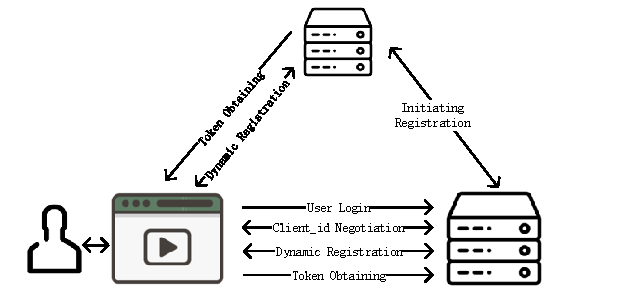
\includegraphics[width=\linewidth]{fig/prioidc.pdf}\label{fig:overview}
  %\subfigure[Authorization Code Flow]{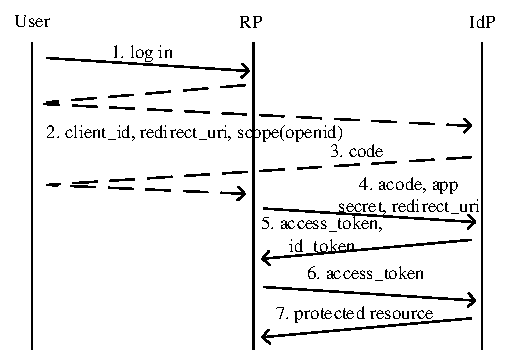
\includegraphics[width=\linewidth]{fig/openidconnect2.pdf}\label{fig:OpenID_code}}
  %\subfigure[Hybrid Flow]{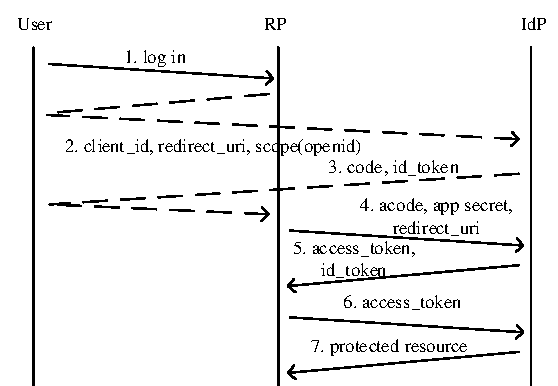
\includegraphics[width=\linewidth]{fig/openidconnect3.pdf}\label{fig:OpenID_hybrid}}
  \caption{Overview of System}
  \label{fig:overview}
\end{figure}
\begin{itemize}
\item[---] Initiating Registration: RPs and users register at IdP. IdP generates unique basic\_client\_id for each RP and unique user id for each user.
\item[---] User Login: User starts log in an RP. If user is labeled as logged in, RP is going to offer service to user. Otherwise RP requires user to start SSO procedure. 
\item[---] Client\_id Negotiation: For each SSO procedure, RP is going to start client\_id negotiation with user. Client\_id is a random number generated by client-id-generating algorithm unrelated with any RP. A client\_id represents login from a user to an RP.
\item[---] Dynamic Registration: To make the client\_id generated by negotiation between user and RP, user is going to register client\_id at IdP by the dynamic registration API provided by IdP. IdP is going to check whether client\_id is unique and ask RP to restart client\_id negotiation for another client\_id.
\item[---] Token Obtaining: After dynamic registration success, RP is going to redirect token request to IdP. IdP firstly authenticates user and then generates id token for RP. Id token contains RP's client\_id and user id. Client\_id is provided by RP and user id is generated through sser-id-generating algorithm by IdP. RP is able to get the constant user identity from user id.
\end{itemize}
 
\subsection{Roles in PriOIDC}
To achieve the goals outlined in Section~\ref{sec:intro}, the requirements and restrictions of abilities owned by each roles in single-sign-on system is defined as following: %要做的内容,总的角色能力描述
\begin{itemize}
    \item \textbf{User} is able to generate RP's client\_id with RP by key data exchanging. User is able to register client\_id in IdP. User is able to modify redirect\_uri in token request and redirect token response to the correct RP's redirect\_uri. User need not to store any data in its computer so that user is able to conduct single sign on in any computer.
    \item \textbf{RP} is able to generate client\_id with user by key data exchanging. RP is able to check the client\_id registration result. RP is able to get a constant user identity from id\_token generated by IdP. RP is unable to find out its user's identity in other RPs even through RPs' collusion. 
    \item \textbf{IdP} is able to generate user's id for specific login by client\_id and user's unique id in IdP. IdP is unable to find out RP's identity by client\_id. IdP is unable to find out the relevance between an RP's  different client\_ids. 
    \item \textbf{User agent} is the software used by the user, such as browser and the application on the mobile device.
\end{itemize}
More detailedly, the enhanced protocol is going to provide new client-id-generating and user-id-generating algorithm: Client\_id is random in each logins to make RP anonymous in IdP. There is a one-to-one correspondence between client\_id and user\_id provided by IdP so that user id is random. So RP is able to transform user\_id IdP into constant user identity and RPs are unable to find the relationship between one user's user\_ids for different RPs. 
\subsection{Threat Model}
Considered different attack scenarios, malicious opponent can be divided into following situations: malicious IdP, malicious RP, malicious user and external attacker. In different situations malicious owns different abilities.
%敌手能力假设:
%作为IdP
%不能够以用户的身份登录RP
%能够获得登录过程中用户的身份信息
%能够获得RP的client_id与redirect_uri信息
%能够长时间留存登录中的信息,并对多次登录信息进行比对
%作为RP
%能够与用户协商client_id
%能够获得用户上传的认证凭据
%能够构造对IdP申请token的请求
%能够获得IdP返回的token
%作为User
%能够与rp协商client_id
%能够篡改经过user转发的数据
%能够构造动态注册的请求
%作为外部攻击者
%能够监听和篡改单点登录过程中的网络流量


\textbf{Curious IdP} As IdP service is usually provided by a leading internet company. In consideration of in consideration of, Idp is considered secure but curious. Phishing attack on IdP is not considered. It means IdP would not try to do the impersonation attack or abduction attack. But an IdP is probably interested in user's login trace in RPs so that it is able to deduce user's interests and behavioral traits. During SSO login, as IdP need authenticate the user, so IdP has the ability to collect the user's information. And IdP is able to get client\_id and redirect\_uri from token request. IdP is also able to store each user's login history and analyze each client\_id and redirect\_uri to find out the relevance among each login.


\textbf{Malicious RP} There are two kinds of malicious RPs. The first is the legal RP owned by malicious opponent and the other is phishing site. Because everyone is able to register as an RP at IdP, it is considered that RP can be fully controlled by malicious. A malicious RP is going to conduct impersonation attack and privacy undermining attack on user. As some attack methods require attacker act as both RP and user, to avoid the repetitive description malicious RP and malicious user is defined: If attacker acts as an RP in attack, attacker is considered as malicious RP. If attacker only acts as a user, it's malicious user. 
A malicious RP's goals include: 1) Getting id\_token from user which is validate in other RPs. 2) Deducing user's login trace by colluding with other RPs. 
Malicious RP is able to make fake basic\_rp\_id and conduct client\_id negotiation with user. Malicious RP is also able to construct the id\_token request to IdP and receive id\_token from IdP. In phishing attack, it is considered that user trusts attacker completely. 


\textbf{Malicious User} A malicious user is only going to conduct impersonation attack. In the attack malicious opponent acts as both user and RP, user is able to conduct client\_id negotiation, construct dynamic registration request. User is also able to temper all the data transformed through itself. It is considered that the user agent is trustful, but there are external attacker trying to exploit the flaw of user agent.


%\textbf{External Attacker} External attacker's targets include impersonation attack, abduction attack and privacy undermining attack. External attacker is able to capture and temper all the network flow through user, RP and IdP. 


